\documentclass{elsarticle}
\usepackage{lipsum}
\usepackage{float}
\usepackage{parskip}
\usepackage{url}
\usepackage{graphicx}
\usepackage{placeins}
\graphicspath{{images/}}

\usepackage[
backend=biber,
style=alphabetic,
citestyle=authoryear
]{biblatex}

\addbibresource{Reference.bib}

\makeatletter
\def\ps@pprintTitle{%
 \let\@oddhead\@empty
 \let\@evenhead\@empty
 \def\@oddfoot{}%
 \let\@evenfoot\@oddfoot}
\makeatother

\begin{document}  
\begin{frontmatter}
\title{Examining the South African Economic and Social Renaissance}


%% Group authors per affiliation:
\author{A. Panko}
\author{G. Harke}
\author{J. Joubert}
\author{K. Hoo}
\author{P. Lee}

\begin{abstract}
The following paper has a look at the historical context of South Africa while attempting to identify key economic drivers. To do this a Random Forest was fit to the data in order to leverage the power of machine learning and determine the feature importance. It was found that Investment GFCF is a key driver and it was confirmed by applying a linear regression in the traditional fashion. 
\end{abstract}

\begin{keyword}
Economics, History, Risk Management, Machine Learning, South Africa
\end{keyword}
\end{frontmatter}

\section{Introduction}
South African history provides great context for a case study in risk management. Analysts have the opportunity to investigate the effects of sociopolitical and economic hardships during the apartheid regime followed by an African Renaissance that has been criticized for implementing so called neo-liberal economic policies (\cite{Mbeki2016a} and \cite{Mbeki2016b}). 

The following sections are split up as follows: section 2 acts as a literature review by analyzing the historical contexts and economic drivers of South Africa's economy. Section 3 summarizes section 2 and discusses the key economic drivers. Section 4 describes the data. Section 5 reviews the methodology of linear regression and random forests in the context of modeling financial time series. Section 6 discusses our findings. Section 7 Concludes.

\section{Historical Context}

% ------------------------------------------------------------------------------------------------
\subsection{The Impact of Apartheid}
After South Africa's all-white National Party gained power in 1948, it began enforcing existing policies of racial segregation under a system called apartheid. Under apartheid, non-white South Africans were forced to live in separate areas from whites and use separate public facilities. Apartheid were implemented for 50 years despite strong oppositions within and outside of South Africa.

\subsubsection{Impact on Economy}
In the two decades following the rise to power of the National Party, whites (particularly Afrikaners) rose above all other ethnic groups in South Africa through their dominant and tactful performance in the labour market. Under apartheid system, black people (greater than 70\% of the population) were pushed to the margins of their land through the imposition of the Land Act of 1913. In result; many blacks are unskilled, illiterate, and have low living standards. Apartheid also attracted sanctions and disinvestment which impacted the South Africa economy on a significant scale especially after mid-1980s.

Back in 1950, South Africa's GDP per capita (ranked 24th) were ahead of countries such as Japan (29th), Turkey (33rd). Based on World Bank’s data available from 1960, it is clear that South Africa's GDP per capita growth were lagging behind these comparable countries during its apartheid period:

\begin{figure}[!h]
    \centering
    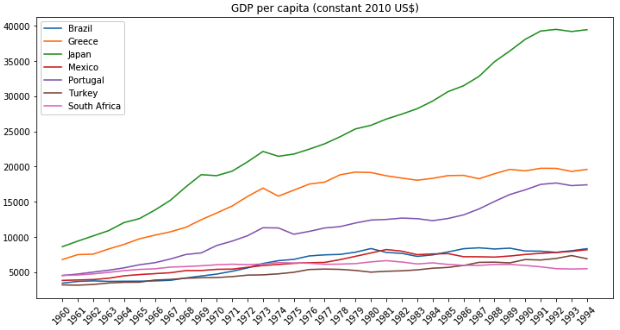
\includegraphics[width=1\textwidth]{images/GDP.jpg}
    \caption{GDP per capita}
    \label{fig:GDP per capita}
    \cite{GDP2019}
\end{figure}

\subsubsection{Impact on Political Landscape}
The apartheid government, under the influence of the ruling National Party, had, by the beginning of the 1980s, divided South Africa into five entities:

\begin{enumerate}
    \item The Republic of Transkei
    \item The Republic of Bophuthatswana
    \item The Republic of Venda
    \item The Republic of Ciskei
    \item The Republic of South Africa
\end{enumerate}

The South African government at the time considered the first four entities to be legally independent countries, but they never received international recognition of their 'statehood'. The international community regarded these four 'republics' as apartheid creatures, the only purpose of which was that of disenfranchising the majority of the citizens of South Africa. In terms of the National Party's ideology, Africans (who constituted close to 80\% of the population of the old South Africa) were supposed to be
citizens of one of these and other potentially 'independent' republics (e.g. one for Zulus in the old Natal Province). They were not entitled to representation in the national parliament.

\subsubsection{Impact on Social Demographics}
Based on Human Development Index (HDI) available from 1990, we are able to compare data from comparable countries for part of the apartheid period until 2008:

\begin{figure}[!h]
    \centering
    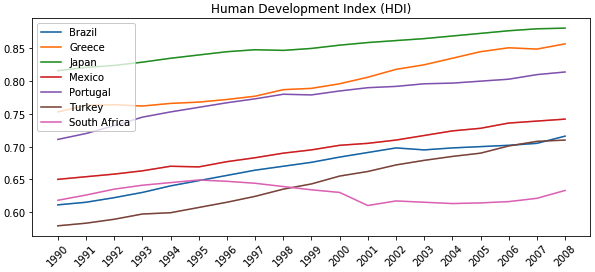
\includegraphics[width=1\textwidth]{images/HDI.jpg}
    \caption{Human Development Index (HDI)}
    \label{fig:Human Development Index (HDI)}
    \cite{HDI2019}
\end{figure}

% ------------------------------------------------------------------------------------------------

\subsection{Cost of Sanctions}
In 1986, South Africa's most important trading partners - (US, EC, Japan) imposed trade and financial sanctions. Specifically:

\begin{enumerate}
    \item Europe and Japan sanctioned import of the Kruger rand and certain steel and iron products
    \item Germany and Great Britain made recommendations and imposed no binding sanctions
    \item US embargoed importing the Kruger rand and certain steel and iron products
    \item OPEC imposed an oil embargo
    \item Europe sanctioned new direct investments but left it to member states to declare if the sanctions would be binding where upon England and Germany did not impose binding sanctions
    \item US sanctioned new direct investments and was the only country to impose sanctions on portfolio investments and credits/loans
\end{enumerate}

Ultimately, the total cost of the trade/financial/oil sanctions were estimated to be 1.5\% with trade sanctions accounting for 1.3\%. During the sanctions period (4th quarter 1986 – 1st quarter 1991) South Africa suffered a net capital outflow of 16.2 billion Rands, which is equivalent to 2\% of GNP (\cite{Hefti2013}). 

Among the list of sanctions, the oil embargo represented the most painful measure for South Africa as it impacted the total population by raising the oil prices whereas it could either gain new trade partners (steel and coal) or modify production (gold bars instead of Kruger Rands) to alleviate the impact of other sanctions

On the other side, the relative meager impact of the financial sanctions was that reinvestment of profits was exempted. In fact, 80\%+ of all FDI in South Africa during that period originated from reinvested profits and reinvested profits by 3 billion Rands during the sanctions which demonstrates investors had maintained a certain trust in South Africa. (\cite{Hefti2013}).

\subsubsection{Analysis}
``Even in the absence of sanctions, apartheid ultimately would have collapsed due to the economic stresses of a hugely inefficient system. Although sanctions may have hurried this process, they were not the driving force behind it. The fall of apartheid was not engineered by foreigners, nor was it primarily precipitated by foreign sanctions'' (Lowenberg and Kaempfer 1998). 

On its face, this was a human rights issue; in reality it may have been closer to culmination of socioeconomic realities and geopolitical evolution of the times. First, the decline of communist regimes lessened the political importance of the South African government as a hedge against communist stronghold in Africa. 

Second, the socio-economic stimulus had been brewing with urbanization of the labor force and limitations of segregated development zones inherent in Apartheid. This limited the existing system as a viable economic solutions in an integrated economy.

As Game-theoretic models (\cite{Kaempfer2007}) suggest, success of sanctions depends on conflict expectations and levels of commitment of the participating nations. From this perspective, sanctions were limited as they were designed with domestic policies in mind and often continued ongoing economic trends. This is shown in that:

\begin{enumerate}
    \item The net outflow of foreign investment was highest in 1985 which one year before imposition of economic sanctions.
    \item US call for coal import sanctions among its partners would have benefited the US coal industry as US and South Africa were competitors for the European coal market.
\end{enumerate}

% ------------------------------------------------------------------------------------------------
\subsection{Privatization in South Africa Post 1994}
The post apartheid new government inherited big debts and over 300 state-owned enterprises and that guzzled subsidies and, for the most part, offered rotten service at extortionate prices.
1994 government was not in favor of privatization.Rather it followed Public Private Partnership model by selling equity to ``strategic equity partners'' and Black Empowerment Groups while retaining a majority interest (\cite{Jerome2004}). 

Privatization aim was to reduce public borrowing, attract foreign investment, promote industrial competition and fuel economic growth.

\subsubsection{Evaluation}
Privatization had many obstacles. Most public firms were in a mess, over-staffed and deep in debt in 1994. The government reckons, for instance, that 27'000 jobs need to be lost at Transnet, the state transport company, and 10'000 at Telkom. Potential investors preferred the government to do this work. Due to high unemployment, government delayed the initiative. South Africa's powerful trade unions were another problem. Their frequent strikes—which brought many public services to a halt and deter investors (\cite{Economist1999}).

Also government was having conflicting view and aims on privatization. One side, it was trying for privatization to raise money and bring in private-sector and foreign expertise. On other side it was seeking public firms to extend services to poor (usually black) areas, which the private sector might ignore(\cite{Hentz2000}). 

Johannesburg Stock Exchange (JSE) supposed to contribute in structural shift to economy with help of financial institutions but due to liquidity and extensive cross holding it didn't contribute much. 

In broader view, the program has not achieved much. Large number of state owned enterprises running businesses.The program didn't deliver much in the area of black economic empowerment. 

Privatization in South Africa had been slow, with few visible results.

% ------------------------------------------------------------------------------------------------
\subsection{Reconstruction and Development Programme (RDP)}

In 1994, Nelson Mandela government developed Reconstruction and Development Programme (RDP) framework in South Africa. A special ministry was established under Jay Naidoo to put initiative in place (\cite{OMalley1998}).

\subsubsection{Objectives}
The RDP emphasized two objectives: the reconstruction of the country and the alleviation of poverty. The RDP's goal was to assist government in integrating growth with social development and economic reconstruction (\cite{Besada2007}).

The RDP framework proposed five suggestion for economic growth: 
\begin{enumerate}
    \item Human resource development
    \item Meet basic necessities
    \item Inject democracy
    \item Public private partnership projects
    \item Boost economy
\end{enumerate}

\subsubsection{Evaluation}
The RDP displayed a dual character. First, as a policy framework, increase donor aid and shrink government's spending. It helped to addressing poverty in states. Also, less funding for military and more funds were allocated to resolve social inequalities in different areas. 

At the same time, RDP fund was established to finance high-profile 'presidential projects', such as public works projects for unemployed youths, free medical care for pregnant mothers, and the electrification of homes of the poor in townships and rural villages. Between April 1994 and December 1998, government built approximately 500 new clinics, which served the health care needs of potentially five million individuals. Through vaccination programs, measles and polio were eradicated(\cite{Besada2007}).

% ------------------------------------------------------------------------------------------------
\subsection{Growth, Employment and Redistribution (GEAR)}
GEAR is a long term, 5 year, macroeconomic policy used to achieve the goals set out in the basic policy framework of the RDP. The reason for the additional policy was because the RDP failed to boost economic growth due to its lack of skilled managers in government, and a narrow focus on fiscal prudence and the reallocation of existing revenues (\cite{SAHO2014}). 

At the time (1996), projected economic growth was 3\%, this would lead to a failure which:
\begin{enumerate}
    \item Would not be able reverse the unemployment crisis
    \item Provided inadequate resources for the expansion of social service delivery
    \item Too slow for an equitable distribution of income and wealth
\end{enumerate}

\begin{table}[H]
  \centering
  \caption{Economic Forecast from 1996, Before GREAR}
  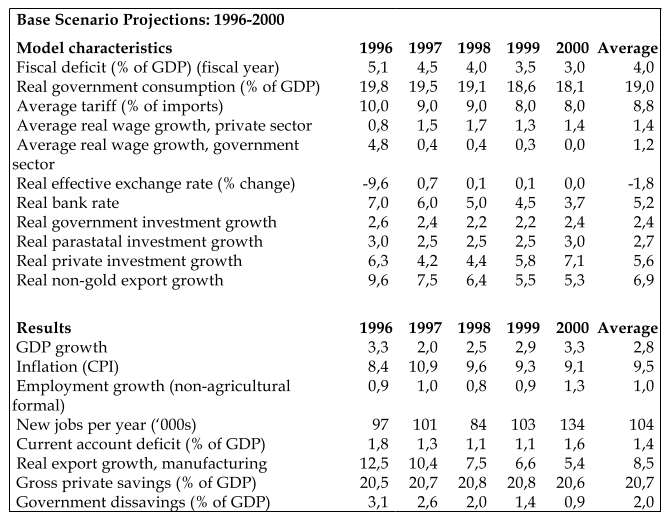
\includegraphics[width=1\textwidth]{images/BeforeGEAR.png}
  \cite{GEAR1996}
\end{table}

Hence the need for a long term macroeconomic policy to boost economic growth to 6\% per annum. This would lead to an additional 400’000 jobs per year until the year 2000.

The GEAR policy would focus on the following points mentioned in (\cite{GEAR1996}):
\begin{enumerate}
    \item Accelerated growth of non-gold exports
    \item Expansion in private sector capital formation
    \item Public sector investment
    \item Employment intensity of investment and output growth
    \item Increase in infrastructure development and service delivery. 
\end{enumerate}

\begin{table}[H]
  \centering
  \caption{Economic Forecast from 1996, With GREAR}
  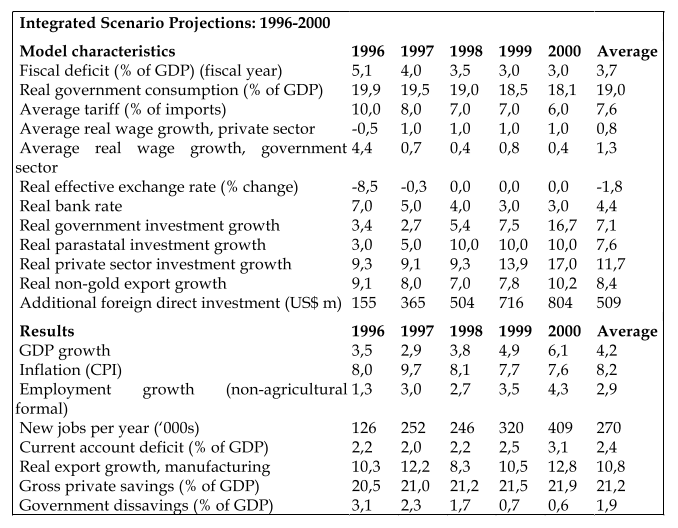
\includegraphics[width=1\textwidth]{images/Gear.png}
  \cite{GEAR1996}
\end{table}

GEAR was also focused on (\cite{SAHO2014}): 
\begin{enumerate}
    \item Reducing fiscal deficits
    \item Lowering inflation
    \item Maintaining exchange rate stability
    \item Decreasing barriers to trade
    \item Liberalizing capital flows
\end{enumerate}

In many ways GEAR was successful in that consumption targets were almost met with the addition of greater macroeconomic stability, better reporting, accountability, and the management of public finances improved. It was also successful in that it reversed the the negative growth rate of the early nineties (\cite{SAHO2014}).

However GEAR was criticized largely by the Congress of South Africa's Trade Unions (COSATU) for its neo-liberal approach which they consider to be in stark contradiction to the RDP, which lead to the ANC party neglecting to implement their nationalisation policies.

GEAR resulted in low levels of economic growth and private investment which led to a disappointing unemployment rate. The policy also failed to redistribute wealth which can be seen in South Africa’s shocking Gini Coefficient of 0.65, 2nd highest in the world! (\cite{WorldBank2014})

In 2005 GEAR was replaced with the Accelerated and Shared Growth Initiative for South Africa (ASGISA)

% ------------------------------------------------------------------------------------------------
\subsection{President Thabo Mbeki (1999 - 2008)}
Thabo Mbeki was South Africa's second post apartheid president, serving from 1999 up to 2008 at which point he resigned shortly before the end of his second term, as he was recalled by the National Executive Committee (NEC) of the ANC.

Mbeki was famous for implementing policies such as (NEPAD, OAU, and the AU) and became known as the “quintessential African nationalist” after Professor Adam Habib declared so in (\cite{Economist2006}). It was noted that his main goal was “to establish the new South Africa as, first and foremost, a black African country” (\cite{Economist2006})

As mentioned previously GEAR was largely criticized by COSATO as being a neo-liberal structural adjustment program. 

In 2016 Mbeki published a letter titled GEAR and Neo-Liberalism in which he defends his stance in a lengthy essay. He concludes the following: “During the whole period when GEAR has been challenged “from the left”, the assertion was made that GEAR sought to replace the RDP. I am certain that there is no rational presentation that can be made to prove this assertion. Alternatively there is no credible argument that can be presented which shows that in the policies and programmes Government actually implemented, once GEAR was adopted it abandoned the pursuit of the RDP objectives.” (\cite{Mbeki2016a} and \cite{Mbeki2016b})

Mbeki was known for reducing state spending however in 1999 he became involved in the now famous arms deal which cost the South African tax payer dearly and was in contrast to his original stance of reducing government spending. (\cite{SAHO2017})

Another scandal during this time was the German Frigate Consortium which saw the people of South Africa purchase 4 new war ships, each worth R4-billion. It was later revealed that a bribe of R130 million was paid to South African politicians. 

% ------------------------------------------------------------------------------------------------
\subsection{Accelerated and Shared Growth Initiative for South Africa (ASGISA)}	
The Accelerated and Shared Growth Initiative for South Africa (ASGRISA) was launched by Deputy President Phumzile Mlambo-Ngcuka in February 2006. The target was halving unemployment and poverty between 2004 and 2014. This could be achieved if the economy grew at an average rate of at least 4.5\% in the period to 2009, and by an average of 6\% in the period 2010 to 2014.

To achieve the objectives of ASGISA there was a need to address some key constraints in the economy. These included the relative volatility of the currency, the cost, efficiency and capacity of the national logistics systems, shortages of suitably skilled labour, and barriers to entry, limits to competition, the regulatory environment, and deficiencies in state organisation, capacity and leadership.
 
Some broad policy areas had been identified as main pillars for ASGISA to accelerate economic growth, including macroeconomic issues, infrastructure investment, education and skills development, industrial and sector strategies, second economy Initiatives, governance and State capacity Issues.

The start in 2006-2007 was promising: investments and public sector infrastructure expenditure increased. Many infrastructure projects were started. Unemployment rate was decreased due to creation of additional job places.

However, in 2007/2008 international financial crisis came. Additionally the administration in South Africa changed. These two factors made ASGISA being confined to the rubbish bin. Zuma administration simply closed ASGISA.

% ------------------------------------------------------------------------------------------------
\subsection{National Development Plan (NDP)}
The National Development Plan 2030 is an important policy document designed by the National Planning Commission. The Commission is an advisory body first constituted in 2009 by President Jacob Zuma. The Plan consists of proposals which are supposed to eliminate poverty and reduce inequality by 2030.

The plan was created to create a country where everyone embraces their full potential, a country where opportunity is determined not by birth, but by ability, education and hard work without existed poverty and inequality. It is clear that the progress in any one area depends on development of another. This means that to achieve these goals the economy must grow faster and at the same time there must be no corruption and crime and so on. That is why the plan includes action across all sectors of South African society. There were nine primary challenges in the main focus:

\begin{enumerate}
	\item Too few people work
	\item The quality of school education for black people is poor
	\item Infrastructure is poorly located, inadequate and under-maintained 
	\item Spatial divides hobble inclusive development
	\item The economy is unsustainably resource intensive
	\item The public health system cannot meet demand or sustain quality
	\item Public services are uneven and often of poor quality
	\item Corruption levels are high
	\item South Africa remains a divided society. 
\end{enumerate}

The plan proposed reasonable actions for every of these areas, however, unfortunately, NDP went the same way as GEAR and ASGISA. All the ideas were great but have not been implemented and goals were not achieved. The plan was too broad, financial crisis played its role and as was written in the plan: ``Its success will depend on all South Africans taking responsibility for the plan, led by the President and Cabinet''.  However, such type of assumptions are to strong for the real life. It's impossible to fight all problems at the same time being too optimistic about the people and the world itself.

% ------------------------------------------------------------------------------------------------
\subsection{Stock Market Developments}
Based on World Bank data available from 1975 on value of stocks traded as \% of GDP, we compared the South Africa's metrics against list of comparable countries (based on similar GDP per capita during 1950). As illustrated below, the stock market capitalization of South Africa grew exponentially post the apartheid era and became comparable to developed country like Japan in terms of its market capitalization to GDP ratio.

\begin{figure}[!h]
    \centering
    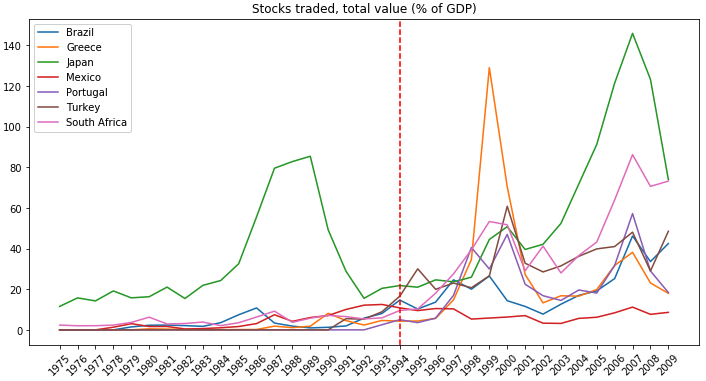
\includegraphics[width=1\textwidth]{images/stock.jpg}
    \caption{Stocks Traded as a Total Value Percentage of GDP}
    \label{fig:Stocks Traded as a Total Value Percentage of GDP}
    \cite{stockstraded}
\end{figure}

South Africa stock market was worth close to twice the country's GDP, which was larger in proportion to most of the emerging countries. The currency, bond and derivatives markets are also among the world’s twenty largest by turnover (\cite{Hassan2013}). 

South Africa's Johannesburg Stock Exchange (JSE) was founded in response to the need for capital to fund the mining sector and it developed along with the growth and expansion of the mining industry. On top of equity, bonds, commodity, and foreign exchange, the JSE also permits trading in interest rate derivatives. It has one of the largest number of product lines per exchange than any other derivatives exchange worldwide. Although the South African market is small comparing to the world's major financial centers, it is one of the more significant among the emerging countries.

% ------------------------------------------------------------------------------------------------
\subsection{Global Financial Crisis (GFC)}
The GFC was a crisis in confidence that led to a global credit freeze. This was initiated by a credit boom and housing bubble - partly initiated by the Clinton agenda to increase home ownership during the 1990’s - and worsened by financial product innovations which multiplied risks exponentially.

The chain of events that led to the GFC include:
\begin{enumerate}
    \item Housing bubble
    \item Asymmetric information/moral hazard
    \item Securitization
    \item Off-balance sheet vehicles which allowed institutions to skirt reserve requirements
    \item Rating agencies
\end{enumerate}

\subsubsection{Impact of GFC on South African Economy}
The South African economy was dependent on financial services and export of manufactured goods/primary commodities (gold, platinum and chrome). Ultimately, the GFC resulted in decreased production due to commercial credit/consumer demand reductions. This led to decline of export and import volumes ultimately leading to net capital outflows from the economy.

Financial Indicators reflected such a downturn: Current account balance as a percentage of the GDP increased from 1.1\% 2008 Q4 to 5.8\% 2009 Q2. GDP growth rate decreased from 1.8\% 2008 Q4 to -3.2\% 2009 Q2. Inflation rose to 8.9\% with real unemployment of 32\% (\cite{Ravinder2014}). 

\subsubsection{Specific Sectors}
Impact on mining sector was shown by decrease in global demand and prices for South African mineral products following the GFC due to tighter fiscal policies. For instance, gold price fell from USD 1030 to USD 750 in 2018. Mining decreased 12.8\% between 2008 Q4 and 2009 Q1. Furthermore, any capital improvement was put on hold due to credit reduction (\cite{Nyanjowa2008}).

Macroeconomic imbalance was manifested in 1) decreased capital investment inflow that led to reduced credit availability which was felt most acutely in service sectors associated with debt-driven expenditure such as construction and automobiles, and 2) fall in manufacturing, mining, financial, business, real estate, and wholesale/retail trade that led to reduction in GDP. For instance, GDP decreased 7.4\% in Q1 2009 and 2.8\% in Q2 2009. This led to the first recession in 17 years (\cite{ILO2010}).

However, recession was shallower than expected due to:
\begin{enumerate}
    \item Lack of direct banking sector exposure to problem assets in the US and strong performance going into the GFC
    \item Low oil prices
    \item Growth in construction in preparation for the FIFA World Cup
\end{enumerate}

Unemployment rate rose from 21.9\% in 2008 and 25.2\% 2010. This was felt most strongly in the low-skilled sectors leading to additional social costs. Ultimately, this lead to increased budget deficit and high public debt which recorded a 1\% surplus in 2008 to -7.3\% in 2010 (\cite{Gordhan2010}). 
% ------------------------------------------------------------------------------------------------

\section{Key Economic Drivers}
After 50 years of apartheid, South Africa's growth was severely limited in terms of economic, political, and social demographic development. The post apartheid period, despite Government efforts to privatize the inefficient, heavily indebted state-owned enterprises, proved more than challenging.

Both The RDP and GEAR policies, which were initiated during Mandela’s presidency, aimed to boost economic growth and social development. Sadly both resulted in low levels of economic growth and disappointing unemployment rates - it also failed to redistribute wealth. During Mbeki’s presidency, ASGISA replaced GEAR with the objective to halve unemployment and poverty between the years 2004 and 2014. To accelerate economic growth, ASGISA targeted broad policy areas such as macroeconomic issues, infrastructure investment, education and skills development. 

The start of 2007 was promising: investments in public sector infrastructure expenditure increased and many infrastructure projects were started. The unemployment rate was decreased due to the creation of additional jobs. However, the 2008 Global Financial Crisis came and ASGISA was closed after Zuma started his presidency in 2009. 

South Africa was not as adversely impacted as other nations by the GFC due to decreased exposure to the toxic assets. Given the changes made on the social and economic frontiers, the South African economy appeared to have progressed forward.

\subsection{Structural Advancements}
South Africa has in the two decades since 1994 made large structural advances in 10 key areas, according to a study by Goldman Sachs (\cite{Coleman2013})

\begin{enumerate}
    \item Macro fiscal and monetary balances have improved
    \item Government debt costs have trended lower and foreign reserves have risen
    \item Overall cost of capital has declined
    \item Corporate valuations have improved relative to global peers
    \item Real asset ZAR returns have compared favourably
    \item China and African trade rise has largely offset European trade decline
    \item Disposable income of South Africans has risen
    \item The rise of the black middle class has led to a structural boost in spending
    \item Wage inflation and government grants have supported this trend
    \item Per unit labour productivity has improved
\end{enumerate}

Despite not fully achieving the intended results, the post-apartheid era policies mentioned in this paper are the key drivers which transformed South Africa to achieve a period of economic performance between 1994-2007 where it recorded average GDP growth rate of 3.6\% (vs the 1.4\% between 1980-1994) and lower average inflation of only 6.3\% (vs the 14.3\% between 1980-1994). These policies improved the macro fiscal and monetary balances, reduced government debt costs (from 49.7\% of GDP in 1994 to 28.3\% in 2007) and increased foreign reserves (from US\$3.1bn in 1994 to US\$39.7bn in 2009).

The corporate environment also improved as the overall cost of capital was reduced (from a lending rate of 15.6\% in 1994 to 13.2\% in 2007), stock valuations improved relative to the global peers (from a gap of 15x difference in forward P/E around 2000 period to equal P/E ratio in 2007), and trading with China increased significantly (exports to China increased from 1.5\% to 12\%, imports increased from 5\% to 14\%).

From a social economic perspective, the policies boosted the ratio of middle and upper class (from 48\% in 2001 to 69\% in 2010), and increased the disposable income of South Africans with impressive CAGR of 10\% (from R665bn in 2001 to R1,494bn in 2009).

% ------------------------------------------------------------------------------------------------

\section{Data}
The following data was taken from the Organisation for Economic Co-operation and Development (OECD) database, Quandl, and the World Bank. 

Independent Variables
\begin{enumerate}
    \item Investment (GFCF)
    \item Current Account Balance
    \item CPI (Inflation)
    \item Long-term Interest Rates
    \item M3 Money Supply
    \item Unemployment
    \item Ores and Metals Import
    \item Crop Production (Wheat)
    \item Exchange Rates (USD/ZAR)
    \item Prime Energy
\end{enumerate}

Dependant Variables
\begin{enumerate}
    \item Gross Domestic Product (GDP)
    \item Share Prices (JALSH Index)
\end{enumerate}

\subsection{Feature Engineering}
As with all statistical modeling, variables need to be engineered to allow models to accurately forecast. Two transformations were applied to the data. The first order log difference was applied to: 
\begin{enumerate}
    \item Gold
    \item Exchange Rate
    \item Share Prices
    \item Long term interest rates
    \item M3 Money supply
    \item Unemployment
    \item GDP
\end{enumerate}

The reason for this is to make the data stationary. Prices are log normally distributed and returns are normally. Next we apply Min Max Scaling to the following variables:
\begin{enumerate}
    \item CPI
    \item Ores & metals
    \item Prime Energy
    \item Investment GFCF
    \item Current Account Balance
\end{enumerate}

% ------------------------------------------------------------------------------------------------

\section{Methodology}
Machine learning is starting to build a good reputation in the financial literature as an effective tool. We made use of a Random Forest's (RF) feature importance to help identify the key drivers in the South African economy and Stock Market. After identifying the most important driver, we applied OLS linear regression to analyse the relationship. Our methodology combined the strengths of RF's non-linearity features and OLS's transparency in explaining the relationship between the variables. 

This section will briefly provide a short explanation of both a RF's feature importance and the OLS Linear Regression technique.

\subsection{Linear Regression: Ordinary Least Square (OLS)}
Ordinary least Square is linear regression method. In OLS linear Regression, the goal is to find the line (or hyperplane) that minimizes the vertical offsets. We define the best-fitting line as the line that minimizes the mean squared error (MSE) between our target variable (y) and our predicted output over all samples i in our dataset of size n.

$$MSE = \frac{1}{n} \sum_{i-1}^{n} (y_i - \hat{y}_i)^2$$

Following are the approaches to perform a linear regression model using ordinary least squares:
\begin{enumerate}
    \item Solving the model parameters analytically (closed-form equations)
    \item Using an optimization algorithm (Gradient Descent, Stochastic Gradient Descent, Newton’s Method, Simplex Method, etc.)
\end{enumerate}

\subsubsection{Normal Equation}
The closed-form solution should be preferred for “smaller” datasets – if computing matrix inverse is not a concern. For very large datasets, or datasets where the inverse of $X^\top X$ may not exist (the matrix is non-invertible or singular, e.g., in case of perfect multicollinearity), the GD or SGD approaches are to be preferred (\cite{Raschka2017}). The linear function (linear regression model) is defined as:

$$y = w_{0}x_{0}+w_{1}x_{1}+...+w_{m}x_{m} = \sum_{j=0}^{m} w^\top x$$

where y is the response variable, x is an m-dimensional sample vector, and w is the weight vector (vector of coefficients). Note that $w_0$ represents the y-axis intercept of the model and therefore $x_0=1$. Using the closed-form solution (normal equation), we compute the weights of the model as follows:

$$w = (X^\top X)^{-1}X^\top y$$

\subsection{Assumption in OLS (\cite{DeFusco2007})}
OLS has the next assumptions:
\begin{enumerate}
    \item The regression model is linear in the coefficients and the error term
    \item The error term has a population mean of zero
    \item All independent variables are uncorrelated with the error term
    \item Observations of the error term are uncorrelated with each other
    \item The error term has a constant variance (no heteroscedasticity)
    \item No independent variable is a perfect linear function of other explanatory variables
\end{enumerate}

Traditionally, in quantitative finance linear regression based factor analysis is used to analyse the performance of the factors in different factor models (such as CAPM, French & Fama five factor model). OLS is widely used to model  the risk distribution. We believe this  traditional approach of quantitative finance will help in our analysis to explain the dependent variables GDP & share price. Also, we observed dependent variables, GDP and share price, are linearly correlated with explanatory variables and hence OLS will help us to find best fit values for coefficient to  explain variability in dependent variables. To perform this analysis using linear regression, we have used statsmodels OLS api.

\subsection{Random Forests & Feature Importance}
Random Forest is an ensemble methods that generates many classifiers and aggregates their results. Boosting (\cite{Shapire1998}) and bagging (\cite{Breiman1996}) of classification trees are two common methods. It is used for classification and regression projects and adds randomness by searching for the most important feature among a random subset of features to split a node. Increased randomness can be produced by using random thresholds for each feature rather than searching for the best possible thresholds. A wide diversity results generally produces a better model.

The relative importance of each feature is measured by evaluating how much the tree nodes reduce impurity across all trees in the forest. The score is automatically computed for each feature after training and scaling the results such that the sum of all importance is equal to 1. Increasing the number of features will increase the risk of overfitting. Here, the algorithm randomly selects observations and features to build several decision trees and then averages the results.

Random forest variable importance measures may not be reliable if predictor variables vary in the scale of measurement or number of categories. As an example, if predictors include both sequence data and continuous variables. When subsampling without replacement is used, the resulting variable importance measures can be used reliably (\cite{Strobl2007}). Estimate of error rate is quite accurate, given that enough trees have been grown (otherwise the OOB estimate can bias upward; see \cite{Bylander2002}).

The Hyperparameters in random forest can be used to: increase the predictive power of the model via maximizing number of features or minimizing number of leafs required to split an internal node. It can also make the model faster via increasing the number of processors used and assuring replicability when given definite value of random state and the same hyperparameters as well as the same training data.

Interpretation of the result requires understanding the trade off between bias and variance. For instance, even though the model is predicting the “right” answer on average, higher variance may make it more difficult to trust the prediction. On the other hand, in a low variance-high bias situation, the predictions are biased but may be more closely clustered. The results may be more operationalised if the bias is understood given its consistency.

% ------------------------------------------------------------------------------------------------

\section{Results}
We trained two RF models separately for each of the dependent variables: GDP and Share Prices. Both RF models point to \textbf{Investment GFCF} as the most important feature, with a greater than 0.3 feature importance. Note that all the values sum to 1.

\begin{figure}[!h]
    \centering
    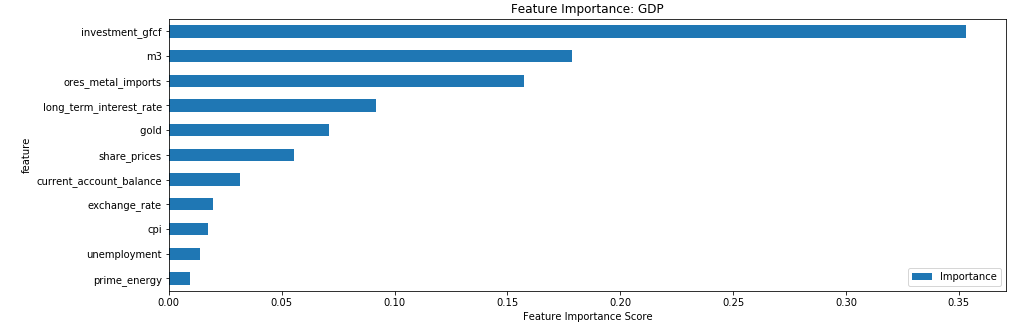
\includegraphics[width=1\textwidth]{images/rf_gdp.png}
    \caption{Feature Importance for GDP}
    \label{fig:Feature Importance for GDP}
\end{figure}

\begin{figure}[!h]
    \centering
    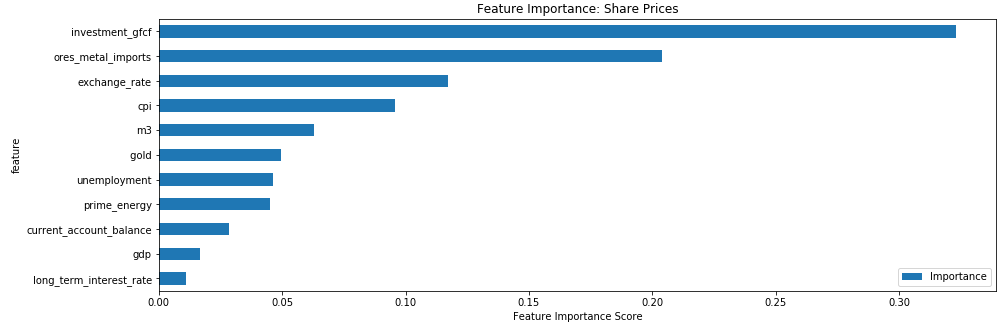
\includegraphics[width=1\textwidth]{images/rf_shares.png}
    \caption{Feature Importance for Share Prices}
    \label{fig:Feature Importance for Share Prices}
\end{figure}

\subsection{Model GDP - Linear Regression}
Next Investment GFCF is used in a traditional linear model. We first perform the analysis on a univariate model on GDP and then Share Prices. Next a multivariate analysis is performed. 

% Graph
\begin{figure}[H]
    \centering
    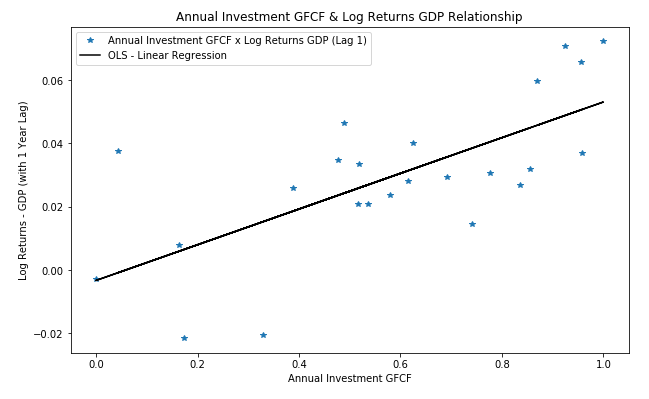
\includegraphics[width=1\textwidth]{images/scatter_1.png}
    \caption{Annual Investment GFCF x Log Returns GDP (Lag 1)}
    \label{fig:Annual Investment GFCF x Log Returns GDP (Lag 1)}
\end{figure}

% Statistics table
\begin{table}[H]
  \centering
  \caption{Model GDP - Linear Regression}
  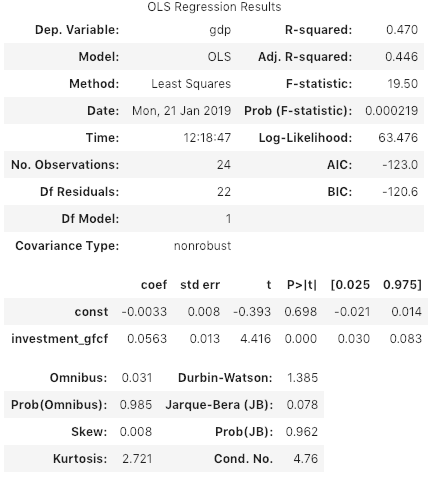
\includegraphics[width=0.7\textwidth]{images/ols_1.png}
\end{table}

As we can see from the graph above, the fitted line reflects the data rather good, for a single variable.
Moreover, the F-statistic and p-value of the coefficient are highly significant. Adjusted R-squared of 0.446, meaning that 44.6\% of the variability of the response data around its mean is explained by the model.

\subsection{Model Stock Market - Linear Regression}
% Graph
\begin{figure}[H]
    \centering
    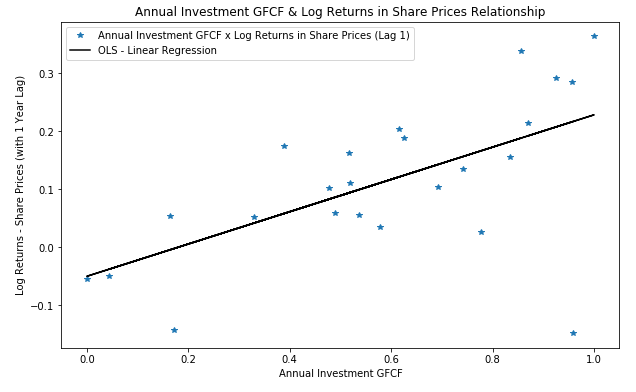
\includegraphics[width=1\textwidth]{images/scatter_2.png}
    \caption{Annual Investment GFCF x Log Returns in Share Prices (Lag 1)}
    \label{fig:Annual Investment GFCF x Log Returns in Share Prices (Lag 1)}
\end{figure}

% Statistics
\begin{table}[H]
  \centering
  \caption{Model Share Price - Linear Regression}
  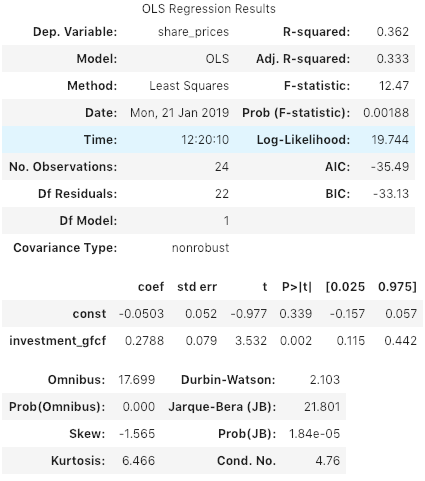
\includegraphics[width=0.7\textwidth]{images/ols_2.png}
\end{table}

For Share Price, however, the model is not as good as before. With the Adjusted R-squared at 0.333.

\newpage
\subsection{Model GDP with All Features}
\begin{table}[H]
  \centering
  \caption{Model GDP with All Features - Linear Regression}
  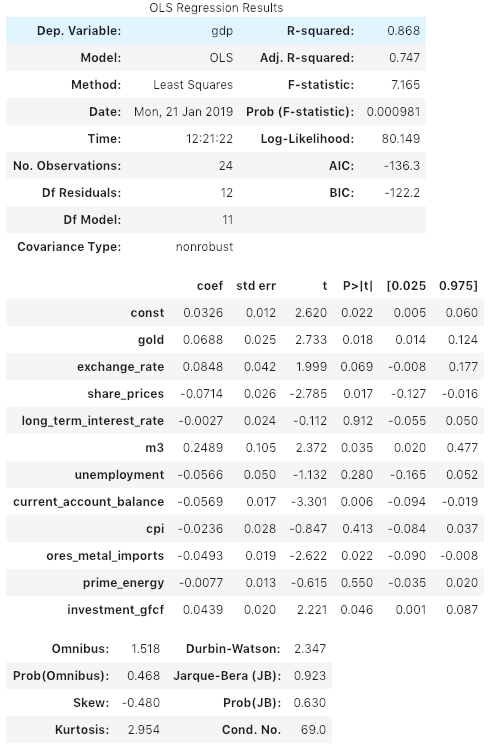
\includegraphics[width=0.7\textwidth]{images/ols_3.png}
\end{table}

\subsection{Model Stock Market with All Features}
\begin{table}[H]
  \centering
  \caption{Model Share Price with All Features - Linear Regression}
  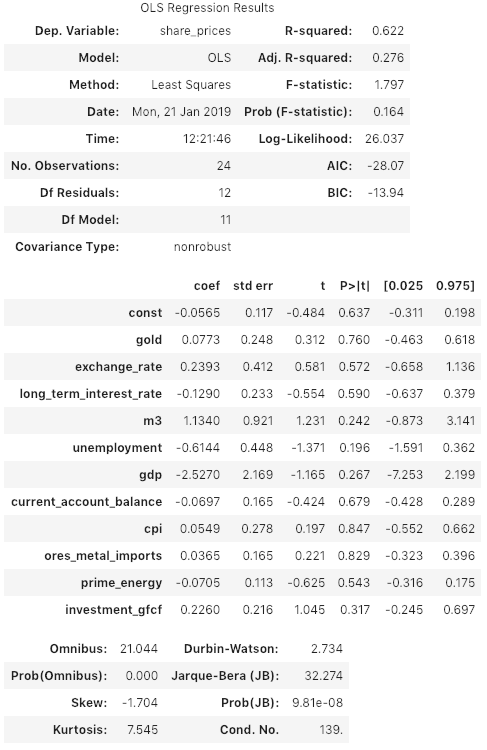
\includegraphics[width=0.7\textwidth]{images/ols_4.png}
\end{table}

The following table does a comparison of multivariate and univariate r-squared values.
\begin{table}[H]
  \centering
  \caption{Comparison of Multivariate and Univariate}
  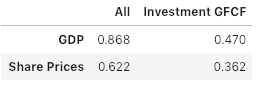
\includegraphics[width=0.5\textwidth]{images/r_square.png}
\end{table}

\section{Conclusion}

We applied Random Forest Regressor (RF) on the 10 selected key factors to model against GDP and Share Prices as proxies to portfolio risk. The RF identified Investment GFCF as the most significant feature (importance scores close to 0.35 for both GDP and Share Prices).

We then applied Ordinary Least-Squares (OLS) Regression on Investment GFCF as a factor on both GDP and Share Prices. For GDP (logged returns with 1 year lag), the OLS model achieved an R-Squared (i.e. the coefficient of determination) of 47\% with just Investment GFCF as input factor. The Share Price model achieved a lower R-Squared score of 36.2\%.

We also illustrated the relationship of the Investment GFCF factor and GDP, Share Prices returns in 2 separate charts together with the corresponding regression lines. 

We compared the performance of our single-factor OLS models against models trained with all 10 initial factors. As seen in table 7 above, although the R-Squared scores are more impressive from the all-factors OLS models, our single-factor models still model relationships reasonably well for just a single variable (R-Squared of 36.2\% for Share Prices and 47\% for GDP)

\printbibliography

\end{document}